\section{Simulation Model Sheets}
\label{app:simfigs}
The scenarios run on every model are S1 (loop closure on the open-loop residual), S3 (module 3 loses a third of its current), S4 ($+1\V$ step on the $\vd{}_{,2}$ reference) and S5 (the open-loop duty steps as sent on the bench), each at $k = 0.1$, 0.2, 0.3, 0.5 and 1 on the bench and solar plants: 28 analytical, 25 QSPICE and 25 carpark-twin runs. Their metrics are in \cref{app:synth}; \cref{fig:twin_sim,fig:qspice_run} show representative runs, and all figures are regenerated by \code{make all} in \code{8\_Results/analysis}.

\begin{figure}[htbp]
  \centering
  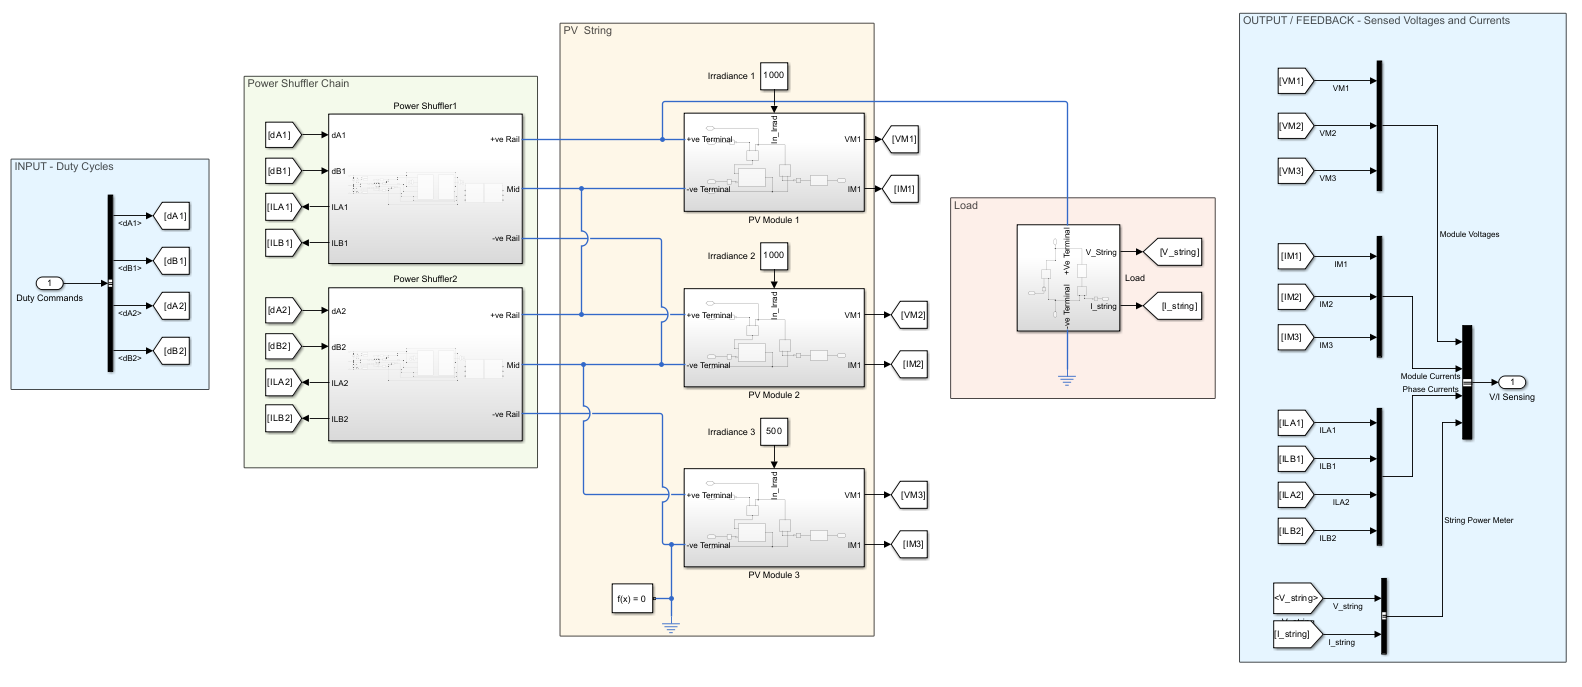
\includegraphics[width=0.95\linewidth]{img-020-036}
  \caption[{Simulink carpark twin}]{Simulink carpark twin: three modules, two averaged-switch shufflers, the sensing block (noise and delay) and the DL3021 CV load. The power-source and load variants are in \cref{fig:twin_variants}.}
  \label{fig:twin}
\end{figure}

\begin{figure}[htbp]
  \centering
  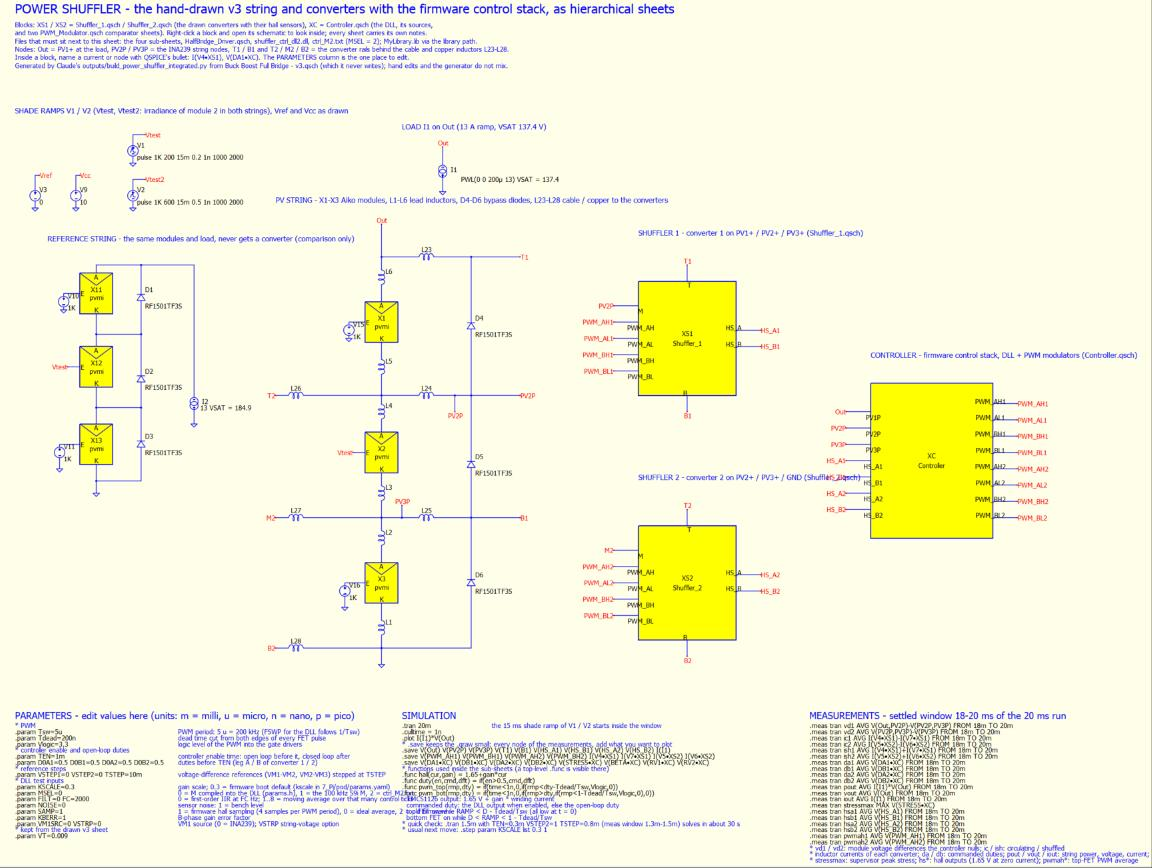
\includegraphics[width=0.8\linewidth]{img-021-041}
  \caption[{QSPICE integrated model, top sheet}]{QSPICE integrated model, top sheet: PV string, two shufflers with real switches, drivers and dead time, and the controller. The controller sheet with the firmware DLL is in \cref{fig:qspice_ctrl}.}
  \label{fig:qspice}
\end{figure}

\begin{figure}[htbp]
  \centering
  \begin{subfigure}[b]{0.45\linewidth}\centering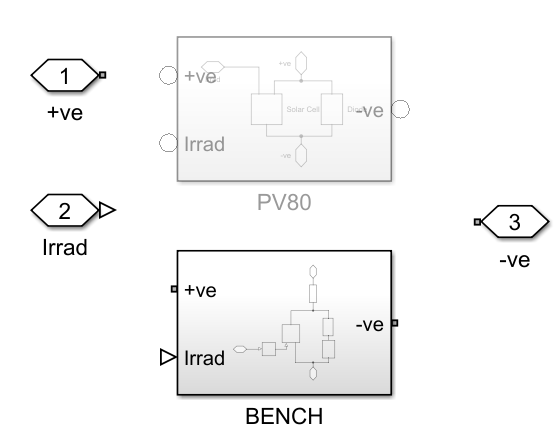
\includegraphics[width=\linewidth]{img-020-038}\caption{Power-source variants (PV80 / BENCH).}\end{subfigure}\hfill
  \begin{subfigure}[b]{0.45\linewidth}\centering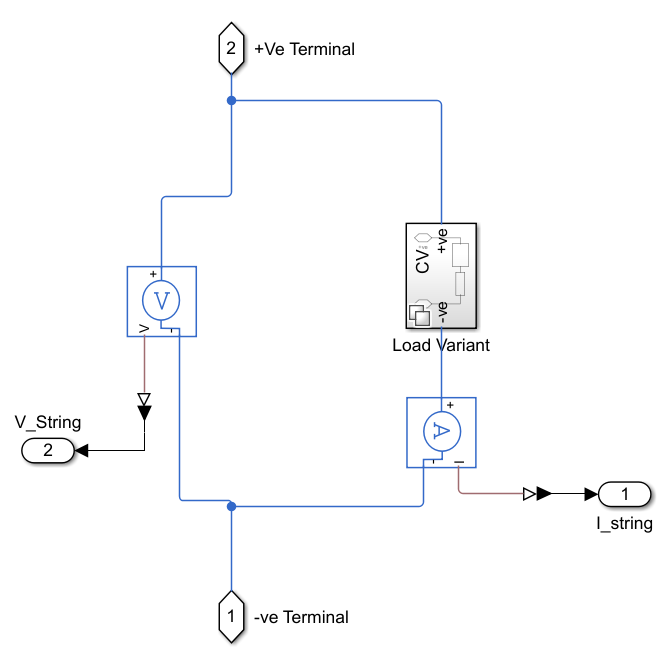
\includegraphics[width=\linewidth]{img-020-039}\caption{Load variants (CV / CC).}\end{subfigure}
  \caption[{Simulink carpark twin: power-source and load variants}]{Simulink carpark twin (\cref{fig:twin}): power-source and load variants.}
  \label{fig:twin_variants}
\end{figure}
\begin{figure}[htbp]
  \centering
  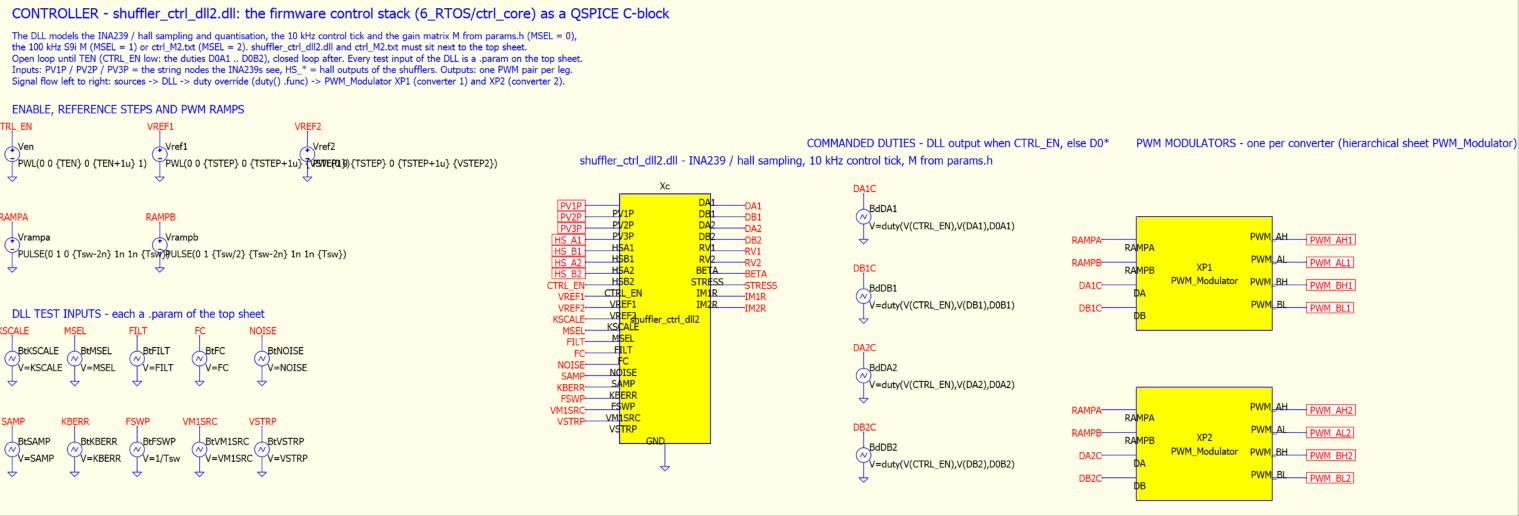
\includegraphics[width=\linewidth]{img-022-045}
  \caption[{QSPICE integrated model, controller sheet}]{QSPICE integrated model (\cref{fig:qspice}), controller sheet: the firmware control DLL (``the Nucleo'') and the HRTIM-style PWM modulators.}
  \label{fig:qspice_ctrl}
\end{figure}
